\documentclass[11pt, a4paper, dvipsnames]{article}

\usepackage{tabularx}
\usepackage{amssymb}
\usepackage[utf8x]{inputenc}
\usepackage[english]{babel}
\usepackage {titlesec}
\usepackage{setspace} \doublespacing

\usepackage [margin=1.2in] {geometry}
\usepackage {amsmath}
\usepackage[T1]{fontenc}
\usepackage{tabto}
\usepackage{ragged2e}
\usepackage{stmaryrd} % for double square brackets

\usepackage{spverbatim}
\usepackage{listings}
\usepackage{multicol}
\usepackage{graphicx}
\usepackage{hyperref}
\usepackage[svgnames]{xcolor}

\usepackage{tikz} 
\usetikzlibrary{positioning}

\newcommand{\upmapsto}{\rotatebox[origin=c]{90}{$\scriptstyle\mapsto$}\mkern2mu} % for coercion

\usepackage{amssymb, upgreek}
\usepackage{mathtools}

\usepackage{color}
\definecolor{keywordcolor}{rgb}{0.7, 0.1, 0.1}   % red
\definecolor{commentcolor}{rgb}{0.4, 0.4, 0.4}   % grey
\definecolor{symbolcolor}{rgb}{0.0, 0.1, 0.6}    % blue
\definecolor{sortcolor}{rgb}{0.1, 0.5, 0.1}      % green
\definecolor{errorcolor}{rgb}{1, 0, 0}           % bright red
\definecolor{stringcolor}{rgb}{0.5, 0.3, 0.2}    % brown

\usepackage{listings}

\titleformat{\section}
{\Large \bfseries}
{}
{1em}
{}

\titleformat{\subsection}
{\large \bfseries}
{}
{1em}
{}

\titleformat{\subsubsection} [runin]
{\normalfont \bfseries}
{}
{0em}
{}

\renewcommand\thefootnote{\textcolor{blue}{\arabic{footnote}}}
\usepackage{perpage} %the perpage package
\MakePerPage{footnote} %the perpage package command

\usepackage{afterpage}
\newcommand\blankpage{
    \null
    \thispagestyle{empty}%
    \addtocounter{page}{-1}%
    \newpage}

\usepackage{tocloft}
\renewcommand\numberline[1]{}

\newcommand{\HRule}[1]{\rule{\linewidth}{#1}}

\usepackage[htt]{hyphenat}
\usepackage{xurl}

\begin{document}

\title{ \normalsize \textsc{}
		\\ [2.0cm]
		\HRule{0.5pt} \\
		\LARGE \textbf{Equivalences of Schema Mappings}
		\HRule{0.5pt} \\ [0.5cm]
		\normalsize  \vspace*{3\baselineskip}}
\date{}
\author{
		4\textsuperscript{th} year project report for candidate 1035522\\
        Honour School of Computer Science - Part C\\
        Submitted as part of an MCompSci in Computer Science\\
		Trinity term, 2022\\ \footnote{Word count: 9364}	
		}

\maketitle
\thispagestyle{empty}
\newpage
\blankpage

\setcounter{page}{3}

\justifying

\section{Abstract}
SHOULD BE A SHORT SUMMARY OF WHAT THE THESIS IS ABOUT, like an abbreviated version of the intro: quickly mentioning what schema mappings, then schema mapping equivalence, then what kinds of problems you study

The majority of computer science areas nowadays deal extensively with different forms of finite relational structures, usually with some form of constraints attached. In the databases domain, we can view the usual relations (tables) as structures, being constrained by dependencies, which impose relationships on the data that can appear in instances. In graph theory, we can view graphs as structures, and the constraints can generate the problems that concern us, for example k-coloring. In this project, we will try to formalize precisely the relational structures and constraints. We will cover a very researched class of constraints, namely tuple-generating dependencies, examining their behavior with respect to database instances. We will also examine how we can decide equivalence of schemas, by imposing conditions on the form of the dependencies.

\section{Acknowledgements}
Many thanks to my supervisor Michael Benedikt for coming up with the idea of the project, for all the help and advice provided, and for constantly bringing up new ideas and methods to solve the problems at hand. His papers and lecture notes constituted the basis for the work of this project, and his weekly meeting notes proved to be essential in progressing with the contributions.

\newpage

\setcounter{secnumdepth}{-1}
\setcounter{tocdepth}{2}
\tableofcontents

\newpage

\section{1. Introduction}
Schema mappings are high-level specifications that describe how to map information from a source schema to a target schema. Logical constraints can be used to represent these relationships, telling how the target must relate to the source. Schema mappings are a crucial building block in several areas of database research, including data exchange\cite{dataexchange}, where we start with data structured under a source schema and we aim to create a target schema that best reflects the input data, and data integration\cite{dataintegration}, where we provide a unified view of all the data from different sources.

\subsection{1.1. Motivation}
In order to describe the relationship between source and target schemas, we use sets of constraints. Naturally, there has been a lot of research on manipulating schema mappings (with operations such as inverse and composition), but this project is focused on the optimization aspect. This consists of the removal of redundant constraints, an operation which can speed up drastically the computation of our target instances. \newline
\textbf{Example 1}: Starting with source database D$_{0}$ = $\{$R(1,2)$\}$ and constraints\newline $\Sigma$ = $\{$R(x,y) $\rightarrow$ S(y,x), S(x,y) $\rightarrow$ R(y,x)$\}$, we would obtain the target instance D$_{0}$ $\cup$ $\{$S(2,1)$\}$, but we can see that the second constraint in $\Sigma$ does not bring any contribution to this, so we could get rid of it.\newline
Using this optimization procedure, we ultimately want to tell if schemas are equivalent (different notions of equivalence will be discussed later). If we possess a repository of schemas which already have some established equivalences between them, this makes querying them more efficient. Consequently, it is important to test any new equivalences that would appear from updating this repository. 

\subsection{1.2. Contributions}
The main goal of this project is to study the relationship between types of equivalences of schema mappings. We will also prove decidability of equivalence testing for particular (and very used in the literature) classes of constraints. This will be done using automata over trees that encode the source instances. Where this decidability has already been proven, our aim is to obtain a better time/memory complexity. In the cases where undecidability has been established, we wish to restrict the class of constraints until the problem becomes decidable. 

\subsection{1.3. Challenges}
The first parts of this project involved getting familiar with the already existing related work, most of it treating similar problems with very different approaches. A crucial concept throughout the project will be the chase procedure, which has been defined in many places and in various ways, therefore trying to encode its structure using graph theory and automata was a big stepping stone. Another challenge arose from the introduction of two new types of equivalences between schemas and our attempt to fit them in the already existing picture of schema equivalences.

\subsection{1.4. Structure of the Report}
The rest of the report is structured as follows: an introduction of the notations and concepts that will be constantly used throughout the project is presented in Section 2.  In Section 3 we introduce the types of equivalences of schema mappings that will be studied, together with how they are related and with decidability results. Section 4 will introduce an approach based on automata which will prove an important result from Section 3. Section 5 will relax one notion of equivalence and will contain decidability results as well. Finally, in Section 6, we present the conclusions, related work and future directions for this project. 

\newpage

\section{2. Preliminaries}

\subsection{2.1. Relational Database Schema}
A \textit{relational schema} S consists of a set of distinct relation definitions (R$_{1}$, R$_{2}$, ..., R$_{n}$), each with an associated "arity". A \textit{relation definition} (also called \textit{table}) consists of its relation name R$_{i}$ and a collection of attribute names paired with their types\newline
(A$_{1}$ : type$_{1}$, ..., A$_{n}$ : type$_{n}$). Since the type of the attributes is not impactful for this project, and for simplicity of definitions, we will mostly use integer types.\newline
A \textit{tuple} (also called \textit{fact}) for a given relation definition R$_{i}$ is a function that assigns to each attribute A$_{i}$ one value from the domain given by its type.\newline
A \textit{primary key} for a table R$_{i}$ is a set of attributes that uniquely determines a tuple in any relation instance (each attribute in the primary key will be underlined). \newline
A \textit{database instance} D$_{0}$ over a schema S consists of one relation instance D$_{0}$(R$_{i}$) for each relation definition R$_{i}$. A \textit{relation instance} for R$_{i}$ is a set of tuples for R$_{i}$ such that no two tuples agree on all the attributes from the primary key of the table.\newline
\textbf{Example 2}: Schema S contains information about a work environment, with one table \textit{EmployeeInfo(\underline{EmployeeID}, Name, Job, Salary)} and one table for structural organization \textit{WorksFor(\underline{EmployeeID}, \underline{BossID})}. The presented database instance only consists of a relation instance for \textit{EmployeeInfo} and has three tuples, with primary key $\{$EmployeeID$\}$.\newline

\begin{tabularx}{0.95\textwidth} { 
  | >{\centering\arraybackslash}X 
  | >{\centering\arraybackslash}X 
  | >{\centering\arraybackslash}X
  | >{\centering\arraybackslash}X | }
 \hline
 EmployeeID & Name & Job & Salary \\
 \hline
 81 & Gilbert Marshall & Reporter & 40000 \\
 \hline
 209 & Jane Hunt & Lawyer & 45000 \\
 \hline
 333 & Neville Barton & Lawyer & 40000\\
 \hline
\end{tabularx} \\

\subsection{2.2. First-order Logic}
Throughout the project we will mostly use \textit{function-free first-order logic} for describing our relation instances, constraints and queries. A \textit{signature} (also called \textit{vocabulary}) for this logic consists of a finite collection of constant symbols and a finite collection of \textit{relations} (also called \textit{predicates}), each having a given \textit{arity}. We can therefore view a relational schema as a signature, and we will use both terms interchangeably. \newline
\textbf{Syntax} : A first-order formula is built from \textit{atomic formulas}, which can either be \textit{relational atoms} R($\vec{t}$), where R is a relation and $\vec{t}$ consists of \textit{terms} (constants or variables), or an equality between two terms. From this, we build formulas inductively using boolean operators ($\wedge, \vee, \neg$) and quantifiers ($\forall, \exists$).
\begin{gather*}
\varphi \hspace{0.5em} ::= \hspace{0.5em} R(\vec{t}) \hspace{0.5em} |\hspace{0.5em} t_{i} = t_{j} \hspace{0.5em}| \hspace{0.5em}\varphi \wedge \varphi \hspace{0.5em}| \hspace{0.5em}\varphi \vee \varphi \hspace{0.5em}| \hspace{0.5em}\neg \varphi \hspace{0.5em}| \hspace{0.5em}\forall x \hspace{0.25em} \varphi \hspace{0.5em}|\hspace{0.5em} \exists x \hspace{0.25em} \varphi\hspace{0.5em}
\end{gather*}
A variable x occurring in a formula $\varphi$ is \textit{bound} if it is in the scope of a quantifier. Otherwise, x is \textit{free}.\newline
Given a signature $\sigma$, we define a \textit{structure} over $\sigma$ to consist of a \textit{domain}, an interpretation for each relation in $\sigma$ as sets of tuples with values from the domain (must preserve the arities), and also an interpretation for each constant symbol in the domain. Thus, we can view an instance I over schema Sch as a structure (Adom(I), R$_{1}$, ..., R$_{n}$), where Adom(I) is the set of values that appear in I and is called the \textit{active domain} of I.\newline
\textbf{Semantics} : For a first-order logic formula $\varphi(\vec{x})$, structure M and function $\sigma$ assigning each variable from $\vec{x}$ to a value in domain(M), we can define inductively on the structure of $\varphi$ the notion of \textit{satisfiability} M, $\sigma \vDash \varphi(\vec{x})$:
\begin{itemize}
	\item M, $\sigma$ $\vDash$ R(x$_{1}$, ..., x$_{n}$) iff $\langle\sigma$(x$_{1}$), ..., $\sigma$(x$_{n}$)$\rangle$ $\in$ M(R);
	\item M, $\sigma$ $\vDash$ x$_{1}$ = x$_{2}$ iff $\sigma$(x$_{1}$) = $\sigma$(x$_{2}$);
	\item M, $\sigma$ $\vDash$ $\varphi_{1}$ $\wedge$ $\varphi_{2}$ iff M, $\sigma$ $\vDash$ $\varphi_{1}$ and M, $\sigma$ $\vDash$ $\varphi_{2}$ (analog for $\vee$ and $\neg$);
	\item M, $\sigma$ $\vDash$ $\exists$ x $\varphi$ iff there is c of type(x) such that M, $\sigma$ $\cup$ $\{x \mapsto c\}$ $\vDash$ $\varphi$ (analog for $\forall$).
\end{itemize}
\textbf{Example 3}: Considering the instance from Example 2, the formula \newline $\varphi$(x, y) = EmployeeInfo(81, x, y, 45000) is not satisfiable by any variable binding, but the formula $\varphi'$(x, y) = EmployeeInfo(81, x, "Reporter", y) is satisfied by the mapping\newline $\sigma$ = $\{$x $\mapsto$ "Gilbert Marshall", y $\mapsto$ 40000$\}$.

\subsection{2.3. Queries}
A \textit{query} is a function mapping instances D$_{0}$ over relational schemas S to relational instances of a fixed relation. If the query has n free variables, then the resulting instance will be n-ary. A \textit{Boolean query} has no free variables and maps instances to either True or False. We will define queries using the function-free first-order logic from above.\newline
To define the particular class of queries that interests us in the project, we recall the fragment of first-order logic called \textit{positive existential} (\textit{$\exists^{+}$}) \textit{first-order logic}, which does not allow the $\neg$ and $\forall$ operators.\newline
\textit{Conjunctive Queries} (CQs) are a fragment of $\exists^{+}$ first-order logic of the form:
\begin{gather*}
Q(\vec{x}) = \exists \vec{y} \hspace{0.25em} \gamma(\vec{x},\hspace{0.25em} \vec{y})
\end{gather*}
where $\gamma(\vec{x}, \hspace{0.25em} \vec{y})$ represents a \textbf{conjunction} of relational atoms that use free variables from $\vec{x}$ and bound variables from $\vec{y}$.\newline
Given instance D$_{0}$ and query Q($\vec{x}$), a \textit{homomorphism of Q in D$_{0}$} (also called \textit{satisfying assignment} or \textit{match}) is a function mapping variables from $\vec{x}$ to values in the active domain of D$_{0}$ that makes Q hold in D$_{0}$. \newline
\textbf{Example 4:} The query Q(x, y) = $\exists z, t_{1}, t_{2} \hspace{0.25em}$ EmployeeInfo(x, y, z, $t_{1}$) $\wedge$ EmployeeInfo(x, y, z, $t_{2}$) will return the following table:\newline

\begin{tabularx}{0.95\textwidth} { 
  | >{\centering\arraybackslash}X 
  | >{\centering\arraybackslash}X | }
 \hline
 209 & Jane Hunt\\
 \hline
 333 & Neville Barton\\
 \hline
\end{tabularx} \\

\noindent Each tuple in the table is a homomorphism of Q in D$_{0}$. We omit the names of the attributes in this project, as we will only care about their position relative to a particular relation name.\newline
A \textit{homomorphism} h \textit{between two structures} D$_{0}$ and D$^{'}_{0}$ (over the same signature) is a function from the active domain of D$_{0}$ to the active domain of D$^{'}_{0}$ such that for every relation R and tuple $\langle$t$_{1}$, ..., t$_{n}\rangle$, we have:
\begin{center}
D$_{0}$ $\vDash$ R(t$_{1}$, ..., t$_{n}$) $\Rightarrow$  D$^{'}_{0}$ $\vDash$ R(h(t$_{1}$), ..., h(t$_{n}$))
\end{center}

\subsection{2.4. Dependencies}
\textit{Dependencies} are integrity constraints over relational database schemas. Intuitively, they are rules to be fulfilled by instances over schemas. Given instance D$_{0}$ and set of dependencies $\Sigma$, we say that D$_{0}$ is \textit{consistent} with $\Sigma$ if it satisfies all constraints in $\Sigma$. All dependencies that we will define will be from fragments of the first-order logic from above.\newline
A \textit{tuple-generating dependency} (TGD) $\varphi$ has the form:
\begin{gather}
\forall \vec{x} \hspace{0.25em}\vec{y} \hspace{0.25em}\rho(\vec{x}, \hspace{0.25em}\vec{y}) \rightarrow \exists \vec{z} \hspace{0.25em}\gamma(\vec{y}, \hspace{0.25em}\vec{z})
\end{gather}
where $\rho$ and $\gamma$ are conjunctions of atoms with arguments from $\vec{x}$ and $\vec{y}$, respectively $\vec{y}$ and $\vec{z}$. Since $\vec{y}$ appears in both sides, these variables will be called \textit{exported variables}. We will refer to $\rho(\vec{x}, \hspace{0.25em} \vec{y})$ as the \textit{body} of the TGD and to $\gamma(\vec{y}, \hspace{0.25em}\vec{z})$ as the \textit{head}.\newline
The intuition behind the "tuple-generating" aspect is that when we start with a database instance D$_{0}$ that does not initially satisfy a TGD $\varphi$ (say we have $\rho(\vec{x}, \hspace{0.25em} \vec{y})$ satisfied, but no $\vec{z}$ such that $\gamma(\vec{y}, \hspace{0.25em}\vec{z})$), we can extend $D_{0}$ with new facts (mentioning new symbols), until we satisfy $\varphi$\footnote{the semantics for TGDs are inherited from first-order logic.}.\newline
\textbf{Example 5}: Consider a database instance $D_{0}$ = $\{$R(0,1), R(1,2), S(0,3)$\}$. The TGD\newline $\varphi_{1}$ = $\forall$x, y S(x,y) $\rightarrow$ $\exists$ z R(x,z) holds, but the TGD $\varphi_{2}$ = $\forall$x, y R(x,y) $\rightarrow$ $\exists$ z S(x,z) does not, because there is no z for x = 1, y = 2 such that S(1,z).\newline
A \textit{guarded tuple-generating dependency} (GTGD) has the form:
\begin{gather*}
\forall \vec{x} \hspace{0.25em}\vec{y} \hspace{0.25em}R(\vec{x}, \hspace{0.25em} \vec{y}) \wedge \rho(\vec{x}, \hspace{0.25em}\vec{y}) \rightarrow \exists \vec{z} \hspace{0.25em}\gamma(\vec{y}, \hspace{0.25em}\vec{z})
\end{gather*}
where R is a relation symbol that mentions all variables from $\vec{x}$ and $\vec{y}$ and is called the \textit{guard} of the constraint. In Example 5, both TGDs are guarded, but for instance the TGD $\varphi$ = $\forall$x, y, z R(x,y) $\wedge$ S(x,z) $\rightarrow$ $\exists$t R(t,x) is not.\newline
A \textit{linear tuple-generating dependency} (LTGD) is a GTGD with only one relation symbol in the body\footnote{some books call it linear guarded TGD, but we can see that all LTGDs are trivially guarded.}:
\begin{gather*}
\forall \vec{x} \hspace{0.25em}\vec{y} \hspace{0.25em}R(\vec{x}, \hspace{0.25em} \vec{y}) \rightarrow \exists \vec{z} \hspace{0.25em}\gamma(\vec{y}, \hspace{0.25em}\vec{z})
\end{gather*}
A \textit{schema mapping} M is defined by a triple $\langle$S, T, $\Sigma\rangle$ where S is the source schema, T is the target schema, and $\Sigma$ is a set of dependencies. Intuitively, $\Sigma$ maps instances of S into instances of T.

\subsection{2.5. Open World Query Answering}
As we have seen, a database instance D$_{0}$ might not be consistent with respect to a set of dependencies $\Sigma$. A natural goal here is to see how to "extend" D$_{0}$ with facts in order for the newly formed instance to satisfy $\Sigma$.\newline
D$^{'}_{0}$ is a \textit{super-instance} of D$_{0}$ if it contains all the facts from D$_{0}$.  Given instance D$_{0}$ and set of constraints $\Sigma$, a \textit{world} (also called \textit{model}) of D$_{0}$ and $\Sigma$ is a super-instance of D$_{0}$ that satisfies $\Sigma$. Given a query Q($\vec{x}$), a \textit{certain answer} to Q on D$_{0}$, $\Sigma$ is a homomorphism h such that the tuple h($\vec{x}$) is in every world of D$_{0}$ and $\Sigma$. \newline
The \textit{Open World Query Answering} problem is to decide, given tuple $\vec{t}$, query Q, instance D$_{0}$ and set of constraints $\Sigma$, whether $\vec{t}$ is a certain answer to Q on D$_{0}$, $\Sigma$. There is a distinction between the constrained and unconstrained versions of this problem, depending if we only take into consideration the finite super-instances or not, respectively. A similar problem is to determine all certain answers of Q, given D$_{0}$ and $\Sigma$.\newline
We will use the notation D$_{0}$ $\wedge$ $\Sigma$ $\vDash$ Q to indicate that Q holds in all possible worlds of D$_{0}$ and $\Sigma$, where Q is a Boolean CQ.\newline
A useful tool in this project is the correspondence between Boolean CQs and databases:
\begin{itemize}
	\item \textbf{Canonical database}: given CQ Q, the canonical database CanonDB(Q) replaces each existential variable in Q with a constant and has one fact for each fact in the body of Q;
	\item \textbf{Canonical query}: given database D$_{0}$, the canonical query CanonQuery(D$_{0}$) replaces each constant from D$_{0}$ with an existential variable and has one atom in the body of the query for each fact in D$_{0}$.
\end{itemize}
\subsection{2.6. Forward Chaining: The Chase}
One common technique for dealing with the open world query answering problem is to derive, given an initial instance D$_{0}$ and set of constraints $\Sigma$, the facts that can be implied in all possible worlds.\newline
Given the TGD $\varphi$ we defined at (1), a \textit{trigger} for $\varphi$ is a  homomorphism h of $\rho$($\vec{x}$, $\vec{y}$) into D$_{0}$. Intuitively, a trigger is simply an assignment of $\vec{x}$ and $\vec{y}$ to values in Adom(D$_{0}$) such that $\rho(\vec{x},$ $\vec{y})$ holds in D$_{0}$. We say that the trigger is \textit{active} if there is no witness $\vec{z}$ such that $\gamma$($\vec{y}$, $\vec{z}$) holds in D$_{0}$, which means that the TGD constraint is not yet satisfied by D$_{0}$.\newline
In order to derive a world where $\varphi$ is satisfied, we create \textbf{new} constants (known as \textit{labelled nulls}) for $\vec{z}$ and we append the necessary facts to D$_{0}$, in order to have a witness for $\gamma$($\vec{y}$, $\vec{z}$). We call this process a \textit{chase step}, and the resulting super-instance will no longer have h as an active constraint. In order to obtain a super-instance which satisfies all constraints from $\Sigma$, we start from D$_{0}$ and make a chase step until there are no active triggers. This procedure will lead to a sequence of instances D$_{0}$, D$_{1}$, ..., D$_{n}$, ..., where each D$_{i+1}$ is obtained from D$_{i}$ by performing a chase step. This is called a \textit{chase sequence} and it can be \textit{terminating} if it is finite and the final instance has no active triggers, otherwise it is \textit{non-terminating}.\newline
For efficiency, we can also act in stages, solving multiple active triggers at once:
\begin{itemize}
	\item Starting from D$_{0}$, apply (in parallel) a chase step for every active trigger and form a super-instance D$_{1}$;
	\item Apply (in parallel) a chase step for each active trigger in D$_{k}$ and form a super-instance D$_{k+1}$;
	\item Continue until there are no active triggers in (say) D$_{n}$
\end{itemize}
This is called a \textit{maximal parallel chase sequence} and we call D$_{n}$ the \textit{parallel chase model}. In case that our process is infinite, we consider as our chase model the direct limit of the structures in it, in our case D$_{0}$, D$_{1}$, ..., D$_{n}$, ..., and we will denote this model as chase$_{\Sigma}$(D$_{0}$).\newline
\textbf{Types of chase}: In the literature, there are multiple ways to define chase sequences, depending on which active triggers are picked. We will mention a few:
\begin{itemize}
	\item \textbf{oblivious chase}: for every pair ($\vec{a}$, $\vec{b}$) and TGD $\varphi$ of the form from (1) with $\rho(\vec{a},$ $\vec{b})$ $\subseteq$ D$_{0}$, apply a chase step to $\varphi$ only if the same pair has not contributed to any previous chase step; therefore, add to D$_{0}$ a new set of atoms $\gamma$($\vec{b}$, $\vec{c}$), where $\vec{c}$ is a fresh set of labelled nulls;
	\item \textbf{restricted chase}: (also called \textbf{standard}) this is a refinement of the previous chase, where we only apply a chase step if the TGD $\varphi$ is not already satisfied by D$_{0}$ i.e. there is no $\vec{a}'$ such that $\gamma$($\vec{b}$, $\vec{a}'$) $\subseteq$ D$_{0}$;
	\item \textbf{super-oblivious chase}: in this variant, we apply chase steps to all matching bodies, no matter if the pair ($\vec{a}$, $\vec{b}$) has been previously used or not.
\end{itemize}
All chase methods can create infinite instances, but it is clear that the restricted chase creates the smallest instances out of the three, and the super-oblivious one the largest.\newline
\textbf{Example 6}: Given the database D$_{0}$ from Example 4 and TGD $\varphi_{2}$, which is not initially satisfied, we can apply one chase step and add a fresh constant null$_{1}$ and the fact S(1, null$_{1}$) to D$_{0}$. Now, the new instance satisfies $\varphi_{2}$ and if we use the restricted or oblivious chase, we would stop here. For the super-oblivious chase, we would add facts S(1, null$_{i}$), for i $\geq$ 1. \newline
\textbf{Properties}: First of all, it is important to notice that the chase procedure will always output a possible world of D$_{0}$ and $\Sigma$, no matter if the procedure is terminating or not. This can easily be deduced from the fact that there will always be a chase step for each active constraint that occurs, which will automatically solve it.\newline
\textbf{Theorem 2.6.1 (Universality Theorem)}.  Given database instance D$_{0}$ and set of constraints $\Sigma$, chase$_{\Sigma}$(D$_{0}$) is a \textit{universal model} for D$_{0}$ and $\Sigma$, meaning that for any world D$^{'}_{0}$ of D$_{0}$ and $\Sigma$, there exists a homomorphism from chase$_{\Sigma}$(D$_{0}$) to D$^{'}_{0}$. \newline
One issue with the chase procedure is that for general TGDs, the termination of the algorithm is undecidable. However, even though for guarded TGDs the chase might be non-terminating, we can decide when to "cut" the procedure, because after some point we no longer obtain new facts (only renamings of the variables).\newline
This crucial theorem will justify the use of the phrase "the chase model", since it implies that for any two chase models, no matter the chase procedure used, there will be a homomorphism between them. Therefore, the chase model is \textit{unique up to homomorphism}. 
The main link to the query answering problem is the following proven result:\newline
\textbf{Corollary 2.6.2.} Consider a set of TGDs $\Sigma$, any database instance D$_{0}$, the chase model chase$_{\Sigma}$(D$_{0}$) and a set of values Base from D$_{0}$ and $\Sigma$. Then, for any CQ Q using only constants from Base, and any tuple $\vec{t}$ with values in Base:
\begin{center}
$\vec{t}$ is a certain answer for Q, D$_{0}$, $\Sigma$ iff $\vec{t}$ is in Q(chase$_{\Sigma}$(D$_{0}$)). 
\end{center}
It has been proven that the problem of finding certain answers is undecidable for the general class of TGDs, but for restricted versions (such as guarded TGDs) this problem is decidable even in the non-terminating case.
\subsection{2.7. Tree-like Property of the Chase}
An important result studied in \cite{decidable} is that the chase procedure for GTGDs is "tree-like". We will present how this result works for LTGDs: 
intuitively, we show that the model can be "coded" as a tree.\newline
Let us fix source instance D$_{0}$ and set of LTGD constraints $\Sigma$. Let the set of constants from D$_{0}$ be Adom(D$_{0}$) = $\{$c$_{1}$, ..., c$_{n}\}$ and the relation names (R$_{1}$, ..., R$_{m}$). Let N = $\{$n$_{1}$, ..., n$_{i}$, ... $\}$ be the set of labelled nulls that will be used in the chase procedure. We represent the chase model of D$_{0}$ and $\Sigma$ as a labelled $\omega$-tree over a set of predicates which will contain all possible facts, combining relation names R$_{i}$ and arguments from Adom(D$_{0}$) $\cup$ N.\newline
\textbf{Example 7}: Let D$_{0}$ = $\{$R(a,b,c)$\}$ and $\Sigma$ = $\{\forall$x,y,z R(x,y,z) $\rightarrow$ $\exists$t R(y,t,x); $\forall$x,y,z R(x,y,z) $\rightarrow$ $\exists$t S(z,t)$\}$. It is clear that the chase procedure here will be non-terminating, since we will always have a new active trigger for each R-fact that is added.\newline 
Formally, we can represent the structure as an infinite labelled tree using the following procedure:
\begin{enumerate}
	\item create a root node and label it with all the facts from D$_{0}$ and mark it as "unexplored";
	\item for each "unexplored" node \textit{v}, let F$_{v}$ be its label (i.e. its set of facts), and let $\Sigma_{v}$ be all the active constraints $\varphi$ from $\Sigma$ such that there exists a fact in F$_{v}$ that is a homomorphism for the body of $\varphi$;
	\item for each such $\varphi$ $\in$ $\Sigma_{v}$, using a chase step we create new facts for each atom in the head of $\varphi$; for each satisfied head we create a new node (which will be a child of \textit{v}) that is labelled with all the new facts (using fresh nulls from N);
	\item mark node \textit{v} as "explored" (the set of "unexplored" nodes acts as the frontier for a BFS-like algorithm);
	\item repeat this process as long as there are "unexplored" nodes; this process might be non-terminating.
\end{enumerate}
\textbf{Example 8}: The labelled tree corresponding to the chase from Example 7 will be:\newline
\begin{center}
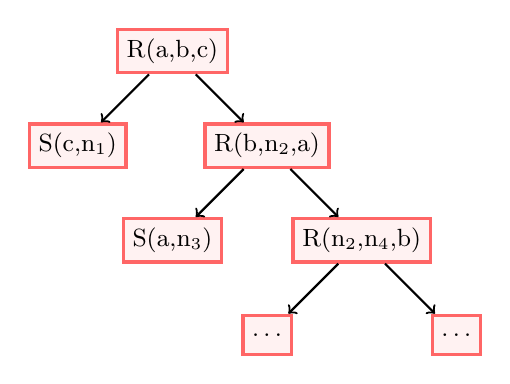
\begin{tikzpicture}[
node distance={17mm}, thick, main/.style = {draw, circle},
squarednode/.style={rectangle, draw=red!60, fill=red!5, very thick, minimum size=5mm}]
\tikzstyle{every node}=[font=\small]
\node[squarednode] (1) {R(a,b,c)}; 
\node[squarednode] (2) [below left of=1] {S(c,n$_{1}$)};
\node[squarednode] (3) [below right of=1] {R(b,n$_{2}$,a)}; 
\node[squarednode] (4) [below left of=3] {S(a,n$_{3}$)};
\node[squarednode] (5) [below right of=3] {R(n$_{2}$,n$_{4}$,b)};
\node[squarednode](6) [below left of=5] {$\hdots$};
\node[squarednode](7) [below right of=5] {$\hdots$};
\draw[->] (1) -- (2);
\draw[->] (1) -- (3);
\draw[->] (3) -- (4);
\draw[->] (3) -- (5);
\draw[->] (5) -- (6);
\draw[->] (5) -- (7);
\end{tikzpicture} 
\end{center}
We can see that N will be infinite, therefore in order to create a labelled $\omega$-tree with finite set of predicates, we need to use a different approach, inspired from \cite{decidable}: \newline
\textbf{Observation}: For every labelled null\footnote{this also holds for constants from D$_{0}$, but not for constants introduced in $\Sigma$.}, the subset of vertices that contain it is connected. \newline
\textbf{Proof}: Suppose there exists a labelled null n such that the set of vertices that contain it is not connected. Therefore, there must be two nodes v$_{1}$ and v$_{2}$ that are labelled with facts that mention n for which no path that connects them exists. For each of the two nodes, we go up the tree as long as the parent of the current node mentions n. We end up with nodes w$_{1}$ and w$_{2}$ which are the ancestors of v$_{1}$ and v$_{2}$, respectively, that are the closest to the root and mention n. If w$_{1}$ = w$_{2}$, then there is a path between v$_{1}$ and v$_{2}$, which leads to a contradiction. If they are distinct nodes, then in both their cases n was introduced by an existential quantifier from an LTGD applied at their parent (w$_{1}$ and w$_{2}$ cannot be root since n must be a labelled null). This implies that the n introduced at w$_{1}$ is distinct from the one introduced at w$_{2}$, as we only introduce fresh nulls each time, which leads to a contradiction.  $\square$\newline
Following this observation, we could re-use labelled nulls in our representation, at the cost of changing their semantics:
\begin{itemize}
	\item Let k be a natural number and L$_{k}$ = $\{$n$_{1}$, ..., n$_{2k}\}$ be a set of labelled nulls (we will call them \textit{local names} to make a distinction from the previous labelled nulls);
	\item When we need to create a new node labelled with S($\vec{x}$, $\vec{y}$), where $\vec{x}$ are bounded and $\vec{y}$ are fresh (with the size of $\vec{y}$ being q), we use the first "available"\footnote{an "unavailable" local name is one used in the parent node.} q local names. 
\end{itemize} 
\textbf{Example 9}: We transform the structure from Example 8 using k = 3 and local names in L = $\{$n$_{1}$, ..., n$_{6}\}$:
\begin{center}
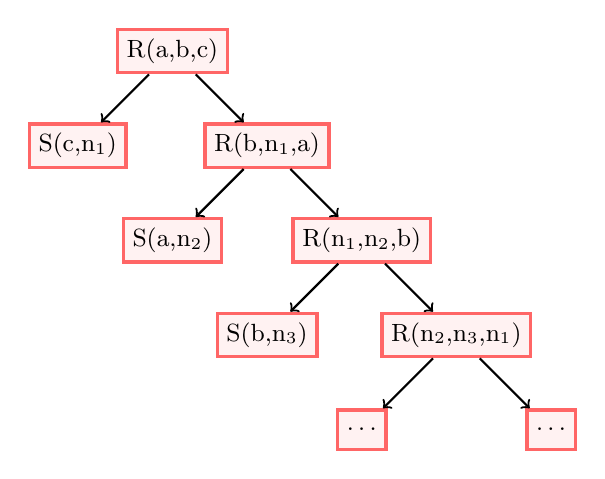
\begin{tikzpicture}[
node distance={17mm}, thick, main/.style = {draw, circle},
squarednode/.style={rectangle, draw=red!60, fill=red!5, very thick, minimum size=5mm}]
\tikzstyle{every node}=[font=\small]
\node[squarednode] (1) {R(a,b,c)}; 
\node[squarednode] (2) [below left of=1] {S(c,n$_{1}$)};
\node[squarednode] (3) [below right of=1] {R(b,n$_{1}$,a)}; 
\node[squarednode] (4) [below left of=3] {S(a,n$_{2}$)};
\node[squarednode] (5) [below right of=3] {R(n$_{1}$,n$_{2}$,b)};
\node[squarednode] (6) [below left of=5] {S(b,n$_{3}$)};
\node[squarednode] (7) [below right of=5] {R(n$_{2}$,n$_{3}$,n$_{1}$)};
\node[squarednode](8) [below left of=7] {$\hdots$};
\node[squarednode](9) [below right of=7] {$\hdots$};
\draw[->] (1) -- (2);
\draw[->] (1) -- (3);
\draw[->] (3) -- (4);
\draw[->] (3) -- (5);
\draw[->] (5) -- (6);
\draw[->] (5) -- (7);
\draw[->] (7) -- (8);
\draw[->] (7) -- (9);
\end{tikzpicture} 
\end{center}
The major difference is that if a local name appears in two different nodes that are not connected in the tree, then the two appearances do not represent the same value.\newline
An important question is what value we should choose for k. Our goal is to minimize its value and consequently the number of possible predicates. As discussed in \cite{decidable}, the optimal value for k is the maximal arity (call it \textit{w}) of any relation in D$_{0}$ or in $\Sigma$.\newline
We need to have at least k $\geq$ \textit{w}, otherwise, if we encounter two facts R(x$_{1}$, ..., x$_{w}$) and R(y$_{1}$, ..., y$_{w}$), where all values mentioned are distinct, we cannot code the values in a consistent way with only 2k local names. In \cite{decidable} we can see that having k = \textit{w} is actually sufficient for every instance that we will encounter.\newline
A crucial point is that every chase structure for source instance D$_{0}$ and set of LTGDs can be represented using this new signature\footnote{in \cite{decidable}, we can find the definition of \textit{k tree-code signature}, a generalization of what we presented here, which is required for a larger class of FO-formulas, called the \textit{Guarded Fragment}.}. 

\newpage

\section{3. Equivalences for the Chase and CQs}
\subsection{3.1. Definitions}
Let us fix a source schema S, a target schema T, and let $\Sigma_{1}$ and $\Sigma_{2}$ be sets of TGD constraints from S to T. We recall three well-studied \cite{equivalence} equivalence types that will be important for the project, together with two more which are \textcolor{red}{newly defined}. 
\begin{enumerate}
	\item \textbf{Logical equivalence}: $\forall$ instances D$_{0}$, D$_{0}$ $\vDash$ $\Sigma_{1}$ iff D$_{0}$ $\vDash$ $\Sigma_{2}$;
	\item \textcolor{red}{\textbf{Chase compatibility}}: $\forall$ source instances D$_{0}$, chase$_{\Sigma_{1}}$(D$_{0}$) $\vDash$ $\Sigma_{2}$ and \newline chase$_{\Sigma_{2}}$(D$_{0}$) $\vDash$ $\Sigma_{1}$;
	\item \textcolor{red}{\textbf{Chase equivalence}}: $\forall$ source instances D$_{0}$, chase$_{\Sigma_{1}}$(D$_{0}$) and chase$_{\Sigma_{2}}$(D$_{0}$) are homomorphically equivalent in both directions (via homomorphisms that preserve the constants in D$_{0}$);
	\item \textbf{CQ-equivalence}: $\forall$ instances D$_{0}$, CQ Q($\vec{x}$), tuple $\vec{t}$ from D$_{0}$, D$_{0}$ $\wedge$ $\Sigma_{1}$ $\vDash$ Q($\vec{t}$) iff D$_{0}$ $\wedge$ $\Sigma_{2}$ $\vDash$ Q($\vec{t}$);
	\item \textbf{DE-equivalence}: $\forall$ source instances D$_{0}$, the models of D$_{0}$, $\Sigma_{1}$ and the models of D$_{0}$, $\Sigma_{2}$ coincide.
\end{enumerate}
The goal of this section is to study the relationship between these types of equivalences and to look at decidability results.
\subsection{3.2. Implications}
For the already known equivalences, the following results hold:
\begin{center}
\textbf{Logical equivalence} $\Rightarrow$ \textbf{DE-equivalence} $\Rightarrow$ \textbf{CQ-equivalence}
\end{center}
We claim the following implications using the new notions:\newline
\textbf{(A) Logical equivalence $\Rightarrow$ Chase compatibility}:\newline
Let D$_{0}$ be a source instance. By the Universality theorem for the chase, we know that chase$_{\Sigma_{1}}$(D$_{0}$) is a universal model for D$_{0}$ and $\Sigma_{1}$, therefore chase$_{\Sigma_{1}}$(D$_{0}$) $\vDash$ $\Sigma_{1}$. Using the assumption, we get that chase$_{\Sigma_{1}}$(D$_{0}$) $\vDash$ $\Sigma_{2}$, too. The other branch is symmetrical.\newline
\textbf{(B) Chase compatibility $\Rightarrow$ Chase equivalence}:\newline
Since chase$_{\Sigma_{1}}$(D$_{0}$) $\vDash$ $\Sigma_{2}$, we have that chase$_{\Sigma_{1}}$(D$_{0}$) is a model (world) for $\Sigma_{2}$. Using the Universality of chase$_{\Sigma_{2}}$(D$_{0}$) for D$_{0}$ and $\Sigma_{2}$, we get that there is a homomorphism from chase$_{\Sigma_{2}}$(D$_{0}$) to chase$_{\Sigma_{1}}$(D$_{0}$). The other direction is symmetrical.\newline
\textbf{(C) Chase equivalence $\Rightarrow$ CQ-equivalence}:\newline
We will do one direction of the iff statement: suppose $\Sigma_{1}$ and $\Sigma_{2}$ are chase equivalent and let instance D$_{0}$, CQ Q($\vec{x}$) and tuple $\vec{t}$. We start with the assumption that D$_{0}$ $\wedge$ $\Sigma_{1}$ $\vDash$ Q($\vec{t}$). From this, we know that Q($\vec{t}$) is a certain answer to D$_{0}$ and $\Sigma_{1}$, therefore Q($\vec{t}$) holds in all possible worlds for D$_{0}$ and $\Sigma_{1}$, one of which is chase$_{\Sigma_{1}}$(D$_{0}$). By chase equivalence, we have a homomorphism
from chase$_{\Sigma_{1}}$(D$_{0}$) to chase$_{\Sigma_{2}}$(D$_{0}$), which preserves every relation and the constants from D$_{0}$. Therefore, it preserves all the CQs, which means that chase$_{\Sigma_{2}}$(D$_{0}$) satisfies Q($\vec{t}$). Using Corollary 2.6.2, we get that D$_{0}$ $\wedge$ $\Sigma_{2}$ $\vDash$ Q($\vec{t}$).\newline
\textbf{(D) CQ-equivalence $\Rightarrow$ Chase equivalence} (in case of \underline{terminating} chase):\newline
Suppose $\Sigma_{1}$ and $\Sigma_{2}$ are CQ-equivalent and let source instance D$_{0}$. We will prove that if the chase procedure for the two sets of constraints terminates, there is a homomorphism from chase$_{\Sigma_{1}}$(D$_{0}$) to chase$_{\Sigma_{2}}$(D$_{0}$) (the other direction is symmetrical). Naturally, chase$_{\Sigma_{1}}$(D$_{0}$) $\vDash$ CanonQuery(chase$_{\Sigma_{1}}$(D$_{0}$)). By CQ-equivalence, chase$_{\Sigma_{2}}$(D$_{0}$) $\vDash$ CanonQuery(chase$_{\Sigma_{1}}$(D$_{0}$)). This means that there is a valuation h$_{12}$ from all the existentially quantified variables in the query to values in the domain of chase$_{\Sigma_{2}}$(D$_{0}$), such that all the facts from the body of the query are satisfied by chase$_{\Sigma_{2}}$(D$_{0}$). Since CanonQuery(chase$_{\Sigma_{1}}$(D$_{0}$)) creates an existential variable for each value in chase$_{\Sigma_{1}}$(D$_{0}$), we can create a homomorphism based on this correspondence and h$_{12}$. This homomorphism will preserve the constants in D$_{0}$.\newline
The new results are:
\begin{center}
\textbf{Logical equiv.} $\Rightarrow$ \textbf{Chase compatibility} $\Rightarrow$ \textbf{Chase equiv.} $\Rightarrow$ \textbf{CQ-equiv.}
\end{center}
We will further investigate the behavior of the equivalences for the class of LTGDs, by giving counter-examples to the reverse direction of some implications:\newline
\textbf{(A') Chase compatibility $\nRightarrow$ Logical equivalence}:\newline
\textbf{Example 10}: Let S consist of unary predicate A(.), T consist of A(.) and unary predicates R$_{1}$(.), R$_{2}$(.). Let:
\begin{itemize}
	\item $\Sigma_{1}$ = $\{$A(x) $\rightarrow$ R$_{1}$(x); A(x) $\rightarrow$ R$_{2}$(x)$\}$;
	\item $\Sigma_{2}$ = $\{$A(x) $\rightarrow$ R$_{1}$(x); R$_{1}$(x) $\rightarrow$ R$_{2}$(x)$\}$.
\end{itemize}
\begin{center}
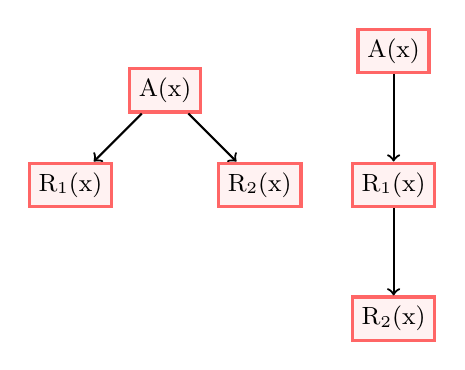
\begin{tikzpicture}[
node distance={17mm}, thick, main/.style = {draw, circle},
squarednode/.style={rectangle, draw=red!60, fill=red!5, very thick, minimum size=5mm}]
\tikzstyle{every node}=[font=\small]
\node[squarednode] (1) {A(x)}; 
\node[squarednode] (2) [below left of=1] {R$_{1}$(x)};
\node[squarednode] (3) [below right of=1] {R$_{2}$(x)}; 
\node[squarednode] (4) [right of=3] {R$_{1}$(x)};
\node[squarednode] (5) [above of=4] {A(x)};
\node[squarednode] (6) [below of=4] {R$_{2}$(x)};
\draw[->] (1) -- (2);
\draw[->] (1) -- (3);
\draw[->] (5) -- (4);
\draw[->] (4) -- (6);
\end{tikzpicture} 
\end{center}
They are chase compatible, as for every source instance D$_{0}$ containing facts of type A(x), we will derive the facts R$_{1}$(x) and R$_{2}$(x). However, they are not logically equivalent, as we have the counter-example D$_{0}$ = $\{$R$_{1}$(0)$\}$, which has D$_{0}$ $\vDash$ $\Sigma_{1}$ and D$_{0}$ $\nvDash$ $\Sigma_{2}$.\newline
\textbf{(B') Chase equivalence $\nRightarrow$ Chase compatibility}:\newline
\textbf{Example 11}: Let S consist of unary relation A(.) and T consist of A(.) plus two binary relations R$_{1}$(. , .) and R$_{2}$(. , .). Let:
\begin{itemize}
	\item $\Sigma_{1}$ = $\{\forall$ w A(w) $\rightarrow$ $\exists$ x, y R$_{1}$(x,y); $\forall$ x, y R$_{1}$(x,y) $\rightarrow$ $\exists$ z R$_{2}$(y,z)$\}$;
	\item $\Sigma_{2}$ = $\{\forall$ w A(w) $\rightarrow$ $\exists$ x, y R$_{1}$(x,y); $\forall$ w A(w) $\rightarrow$ $\exists$ y, z R$_{2}$(y,z); $\forall$ y, z R$_{2}$(y,z) $\rightarrow$ $\exists$ x R$_{1}$(x,y)$\}$.
\end{itemize}
They are chase equivalent and it is easy to create homomorphisms between the labelled nulls of the two structures. For chase compatibility, let D$_{0}$ = $\{$A(0)$\}$. The chases are:
\begin{center}
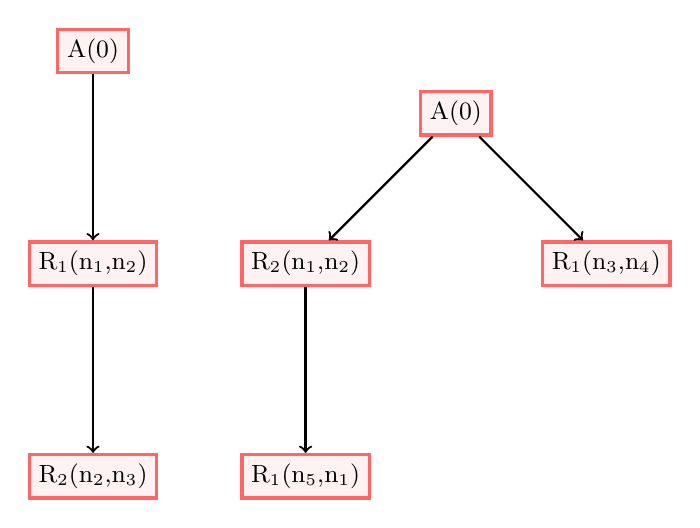
\begin{tikzpicture}[
node distance={27mm}, thick, main/.style = {draw, circle},
squarednode/.style={rectangle, draw=red!60, fill=red!5, very thick, minimum size=5mm}]
\tikzstyle{every node}=[font=\small]
\node[squarednode] (1) {A(0)}; 
\node[squarednode] (2) [below of=1] {R$_{1}$(n$_{1}$,n$_{2}$)};
\node[squarednode] (3) [below of=2] {R$_{2}$(n$_{2}$,n$_{3}$)}; 
\node[squarednode] (4) [right of=2] {R$_{2}$(n$_{1}$,n$_{2}$)};
\node[squarednode] (5) [below of=4] {R$_{1}$(n$_{5}$,n$_{1}$)};
\node[squarednode] (6) [above right of=4] {A(0)};
\node[squarednode] (7) [below right of=6] {R$_{1}$(n$_{3}$,n$_{4}$)};
\draw[->] (1) -- (2);
\draw[->] (2) -- (3);
\draw[->] (6) -- (4);
\draw[->] (4) -- (5);
\draw[->] (6) -- (7);
\end{tikzpicture} 
\end{center}
where chase$_{\Sigma_{2}}$(D$_{0}$) does not satisfy the second constraint from $\Sigma_{1}$, because of R$_{1}$(n$_{3}$,n$_{4}$).\newline
\textbf{Q: Under what conditions does CQ-equivalence $\Rightarrow$ Chase compatibility hold?}\newline
\textbf{Theorem 3.2.1}: Let $\Sigma_{1}$ and $\Sigma_{2}$ be two sets of single-headed\footnote{LTGDs with only one atom in the head : $\forall$ $\vec{x}$,$\vec{y}$ R($\vec{x}$,$\vec{y}$) $\rightarrow$ $\exists$ $\vec{z}$ S($\vec{y}$,$\vec{z}$)} LTGDs with the following properties:
\begin{enumerate}
	\item every constraint mentions only binary predicates;
	\item the body of each constraint has two distinct universally quantified variables;
	\item the head of each constraint contains exactly one exported variable and one existential variable;
	\item the set of constraints does not lead to a chase where there exist a value (constant or labelled null) that appears both in a node and in its grandchild.
\end{enumerate}
Then, if $\Sigma_{1}$ and $\Sigma_{2}$ are CQ-equivalent, then they are also chase compatible.\newline
\textbf{Proof}: \newline
\textbf{Claim 1}: In any chase structure based on this class of LTGDs, if the facts from two distinct nodes share a value, then the relationship between them is either parent-child, or they are children of the same node.\newline
\textbf{Proof 1}: Let n$_{1}$ and n$_{2}$ be such two nodes, sharing value v. Using the connected subset property of the chase, all nodes on the path between n$_{1}$ and n$_{2}$ share v. If the length of the path between them is greater than 2, then there must exist a violation of rule 4. If the distance is 2, then either one node is the grandchild of the other, which is not allowed, or they are the children of the same node. If the distance is 1, we get the parent-child relationship.\newline
From the requirements imposed on the constraints, we can derive their form:
\begin{gather*}
\varphi = \forall x \hspace{0.25em} y \hspace{0.25em} R(x, \hspace{0.25em} y) \rightarrow \exists z \hspace{0.25em} S(y, \hspace{0.25em} z)\\
\varphi = \forall x \hspace{0.25em} y \hspace{0.25em} R(x, \hspace{0.25em} y) \rightarrow \exists z \hspace{0.25em} S(z, \hspace{0.25em} y)\\
\varphi = \forall x \hspace{0.25em} y \hspace{0.25em} R(x, \hspace{0.25em} y) \rightarrow \exists z \hspace{0.25em} S(x, \hspace{0.25em} z)\\
\varphi = \forall x \hspace{0.25em} y \hspace{0.25em} R(x, \hspace{0.25em} y) \rightarrow \exists z \hspace{0.25em} S(z, \hspace{0.25em} x)
\end{gather*}
We will now argue by contradiction. Suppose that the two sets are CQ-equivalent, but there exists a source instance D$_{0}$ such that at least one of the necessary conditions does not hold, say chase$_{\Sigma_{2}}$ $\nvDash$ $\Sigma_{1}$. We denote chase$_{\Sigma_{i}}$(D$_{0}$) as CH$_{i}$, for i $\in$ $\{$1,2$\}$. Therefore, there must exist constraint $\varphi$ $\in$ $\Sigma_{1}$ such that CH$_{2}$ $\nvDash$ $\varphi$. We will say that $\varphi$ is of the form $\forall$x y R(x,y) $\rightarrow$ $\exists$ z S(y,z), but all other cases can be treated the same way. There must exist a witness R(a,b) in CH$_{2}$ such that there is no c with CH$_{2}$ $\vDash$ S(b,c). Let F$_{0}$ = D$_{0}$, F$_{1}$, F$_{2}$, ..., F$_{k-1}$, F$_{k}$ = R(a,b) be the path (in CH$_{2}$) up to this witness.\newline
\textbf{Claim 2}: There must exist a path F$^{'}_{0}$ = D$_{0}$, F$^{'}_{1}$, F$^{'}_{2}$, ..., F$^{'}_{k-1}$, F$^{'}_{k}$ in CH$_{1}$ that is homomorphic (preserving the constants in D$_{0}$) to the given path in CH$_{2}$.\newline
Let R$_{i}$(a$_{i}$,b$_{i}$) be the fact corresponding to F$_{i}$. We know from the given properties of the constraints that precisely one of a$_{i}$ and b$_{i}$ appears in F$_{i-1}$ and the other one is a fresh null. We can form the canonical query Q of the path from CH$_{2}$, which will have as free variables all constants from D$_{0}$ and k universal variables, one for each fresh null introduced by each fact. The CQ-equivalence between $\Sigma_{1}$ and $\Sigma_{2}$ implies that CH$_{1}$ satisfies Q, which in turn implies the existence of facts F$^{'}_{1}$, F$^{'}_{2}$, ..., F$^{'}_{k-1}$, F$^{'}_{k}$ such that F$^{'}_{i}$ shares exactly one value with F$^{'}_{i-1}$, 1 $\leq$ i $\leq$ k. We only remain to prove that these facts form a path in CH$_{1}$, as the part with the homomorphism is proven by the query satisfaction. We will build this path using strong induction on 0 $<$ i $<$ k:\newline
\textbf{Base case}: Because of Claim 1, F$^{'}_{1}$ must be a child of D$_{0}$;\newline
\textbf{Inductive step}: Suppose that F$^{'}_{0}$ = D$_{0}$, F$^{'}_{1}$, F$^{'}_{2}$, ..., F$^{'}_{i-1}$, F$^{'}_{i}$ form a path. Because of Claim 1, F$^{'}_{i+1}$ is either a child of F$^{'}_{i}$, or a child of F$^{'}_{i-1}$, but using the connected subset property for the chase, the latter case will imply that F$^{'}_{i-1}$ contains the value shared between F$^{'}_{i}$ and F$^{'}_{i+1}$, which violates rule 4.\newline
Therefore, F$^{'}_{k}$ will have a fact of the form R(a',b'). Because $\varphi$ $\in$ $\Sigma_{1}$, the chase procedure guarantees that there exist a child F$^{'}_{k+1}$ of F$^{'}_{k}$ that contains the fact S(b',c'), for a fresh null c'.\newline
Now, we can use a similar approach for the path from CH$_{1}$ (augmented with F$^{'}_{k+1}$) to create the canonical query Q', which must be satisfied by CH$_{2}$. Analogously to what we did above and using the same reasoning as for Claim 2, there must exist a path F$^{''}_{0}$ = D$_{0}$, F$^{''}_{1}$, F$^{''}_{2}$, ..., F$^{''}_{k-1}$, F$^{''}_{k}$, F$^{''}_{k+1}$ in CH$_{1}$ that is homomorphic (preserving the constants in D$_{0}$) to the path from CH$_{1}$.\newline
Because of this last homomorphism, F$^{''}_{k}$ must have a fact of the form R(a'',b'') and F$^{''}_{k+1}$ a fact of the form S(b'',c''). The chase procedure guarantees that whenever we have a parent-child relationship, the child was created due to a constraint being applied, therefore we must have a constraint of the same form as $\varphi$ in $\Sigma_{2}$, but this leads to a contradiction, as F$_{k}$ could no longer be a witness that $\varphi$ does not hold in CH$_{2}$.\newline
\begin{center}
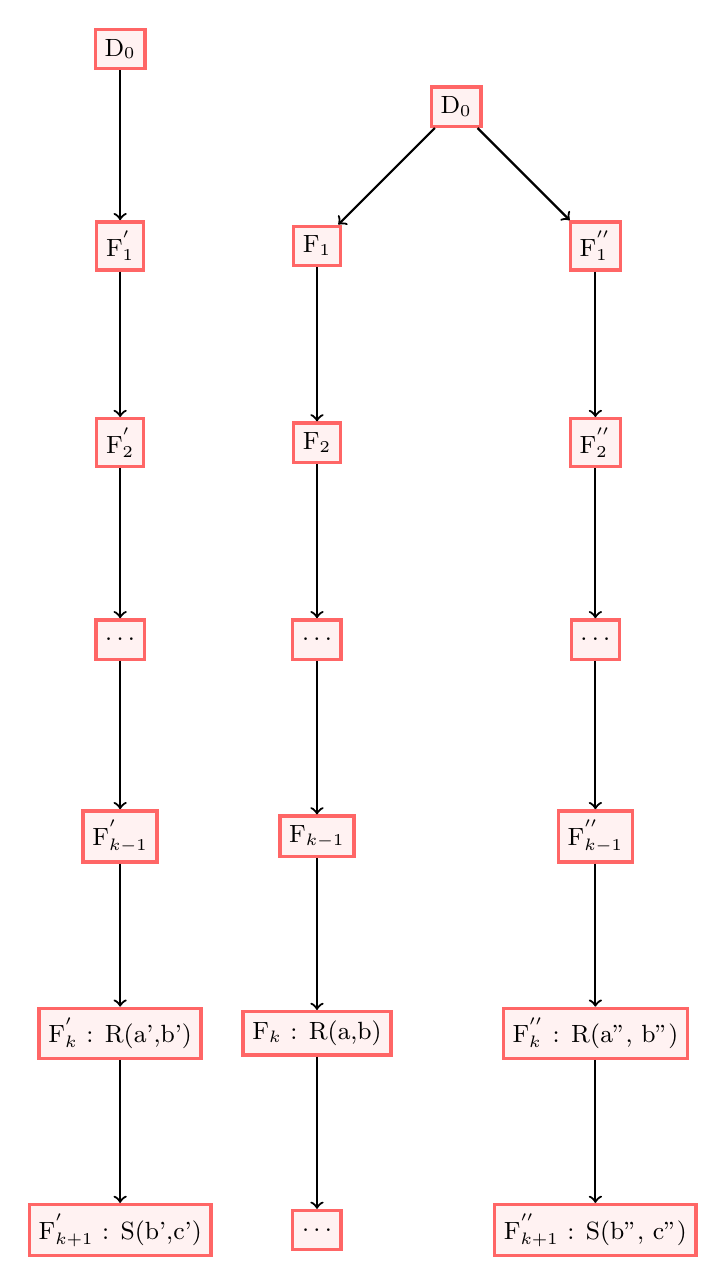
\begin{tikzpicture}[
node distance=2.5cm and 10cm, thick, main/.style = {draw, circle},
squarednode/.style={rectangle, draw=red!60, fill=red!5, very thick, minimum size=5mm}]
\tikzstyle{every node}=[font=\small]
\node[squarednode] (1) {D$_{0}$}; 
\node[squarednode] (2) [below of=1] {F$^{'}_{1}$};
\node[squarednode] (3) [below of=2] {F$^{'}_{2}$}; 
\node[squarednode] (4) [below of=3] {$\hdots$};
\node[squarednode] (5) [below of=4] {F$^{'}_{k-1}$};
\node[squarednode] (6) [below of=5] {F$^{'}_{k}$ : R(a',b')};
\node[squarednode] (7) [below of=6] {F$^{'}_{k+1}$ : S(b',c')};
\node[squarednode] (8) [right of=6] {F$_{k}$ : R(a,b)};
\node[squarednode] (9) [above of=8] {F$_{k-1}$};
\node[squarednode] (10) [above of=9] {$\hdots$};
\node[squarednode] (11) [above of=10] {F$_{2}$};
\node[squarednode] (12) [above of=11] {F$_{1}$};
\node[squarednode] (13) [above right of=12] {D$_{0}$};
\node[squarednode] (14) [below of=8] {$\hdots$};
\node[squarednode] (15) [below right of=13] {F$^{''}_{1}$};
\node[squarednode] (16) [below of=15] {F$^{''}_{2}$};
\node[squarednode] (17) [below of=16] {$\hdots$};
\node[squarednode] (18) [below of=17] {F$^{''}_{k-1}$};
\node[squarednode] (19) [below of=18] {F$^{''}_{k}$ : R(a'', b'')};
\node[squarednode] (20) [below of=19] {F$^{''}_{k+1}$ : S(b'', c'')};

\draw[->] (1) -- (2);
\draw[->] (2) -- (3);
\draw[->] (3) -- (4);
\draw[->] (4) -- (5);
\draw[->] (5) -- (6);
\draw[->] (6) -- (7);
\draw[->] (9) -- (8);
\draw[->] (10) -- (9);
\draw[->] (11) -- (10);
\draw[->] (12) -- (11);
\draw[->] (13) -- (12);
\draw[->] (8) -- (14);
\draw[->] (13) -- (15);
\draw[->] (15) -- (16);
\draw[->] (16) -- (17);
\draw[->] (17) -- (18);
\draw[->] (18) -- (19);
\draw[->] (19) -- (20);
\end{tikzpicture} 
\end{center}

\subsection{3.3. Decidability for Equivalences}
\textbf{(A) Logical equivalence}:\newline
%In \cite{decidable} we are introduced 
%michael: \cite{decidable} did not introduce this logic
We will go through a fragment of first-order logic called the \textit{Guarded Fragment}, where the formulas are of the form:
\begin{gather*}
\varphi(\vec{x}) \hspace{0.1em} ::= True \hspace{0.1em} | \hspace{0.1em} False \hspace{0.1em} | \hspace{0.1em} R(\vec{t}) \hspace{0.3em} |\hspace{0.3em} t_{i} = t_{j} \hspace{0.3em}| \hspace{0.3em}\varphi \wedge \varphi \hspace{0.3em}| \hspace{0.3em}\varphi \vee \varphi \hspace{0.3em}| \hspace{0.3em}\neg \varphi \hspace{0.3em}| \hspace{0.3em}\forall \vec{y} \hspace{0.25em} R(\vec{x}, \vec{y}) \rightarrow \varphi \hspace{0.3em}|\hspace{0.3em} \exists \vec{y} \hspace{0.25em} R(\vec{x}, \vec{y}) \wedge \varphi\hspace{0.3em}
\end{gather*}
In the existential and universal cases, the free variables of the inner $\varphi$ are required to be from $\vec{x}$ $\cup$ $\vec{y}$ and the R($\vec{x}$,$\vec{y}$) atom is called the \textit{guard atom}.\newline
It has been proven that we can construct automata for these formulas in order to decide their satisfiability: see, for example, \cite{decidable}. With this, we can check if two sets of GF formulas are logically equivalent. We can use this approach for GTGD formulas, even when they are not in GF:
\begin{center}
$\varphi$ = $\forall$x, y R(x,y) $\rightarrow$ $\exists$ z S(x,z) $\wedge$ T(y,z)
\end{center}
is not in GF, but we can convert it to GF using a fresh Dummy relation name:
\begin{center}
$\forall$x, y R(x,y) $\rightarrow$ $\exists$ z Dummy(x,y,z)\\
$\forall$x, y, z Dummy(x,y,z) $\rightarrow$ S(x,z)\\
$\forall$x, y, z Dummy(x,y,z) $\rightarrow$ T(y,z)
\end{center}
These formulas are all in GF, and we can do this for any GTGD.\newline
Consequently, \textbf{logical equivalence for GTGDs is decidable}. \newline
\textbf{(B) Chase compatibility}:
This decidability result will be studied in the next chapter, and will require a method of deciding an entailment of the form chase$_{\Sigma}$(D$_{0}$) $\vDash$ $\varphi$.\newline
\textbf{(C) CQ-equivalence}: Under the conditions imposed in Theorem 3.2.1, CQ-equivalence is the same as chase compatibility.  

\newpage

\section{4. Chase Entailment for LTGDs}
In order to prove results for chase compatibility introduced previously, we will use the following:\newline
\textbf{Theorem 4.0.1.} For a fixed instance D$_{0}$, $\Sigma$ a set of single-headed LTGDs and $\varphi$ a single-headed LTGD, we can decide chase$_{\Sigma}$(D$_{0}$) $\vDash$ $\varphi$. \newline
The approach inspired from \cite{decidable} follows the plan:
\begin{itemize}
	\item Show that each such chase structure can be represented by a tree-like model (a structure that can be "coded" in a tree) - Section 2.7;
	\item Create an automata that will accept trees that code the given chase structure - Section 4.2;
	\item Create an automata that will accept only trees that satisfy $\neg \varphi$ - Section 4.4;
	\item Intersect the two automata and check for non-emptiness - Section 4.5.
\end{itemize}

\subsection{4.1. Automata over Infinite Trees: 1-way deterministic Buchi}
We define the type of automaton that is capable of representing the chase model of D$_{0}$ and $\Sigma$: let us fix a maximal outdegree r for the trees that will be considered as input from now on.\newline
\textbf{Definition 4.1.1}: A 1-way deterministic B$\ddot{u}$chi tree automaton is a 5-tuple \newline
$\mathcal{A}$ = $<$Q, Alph, $\delta$, I, F$>$, where:
\begin{itemize}
	\item Q is a finite set of \textit{states};
	\item Alph is an input \textit{alphabet};
	\item $\delta$ : Q $\times$ Alph $\rightarrow$ $\bigcup_{1 \leq i \leq r}$ Q$^{i}$ is the \textit{transition function};
	\item I $\subseteq$ Q is the set of \textit{initial} states;
	\item F $\subseteq$ Q is the set of \textit{final} (also called \textit{accepting}) states.
\end{itemize}
It takes as input an infinite Alph-tree and processes it top-down. A \textit{run} assigns states from Q to the nodes of the tree. A \textit{successful} (or \textit{accepting}) run must satisfy the following conditions:
\begin{itemize}
	\item The root of the tree must be assigned to an initial state from I;
	\item If a node v labelled with $\tau$ and children v$_{1}$, ..., v$_{n}$ is assigned to state q and we have $\delta$(q, $\tau$) = (q$_{1}$, ..., q$_{n}$), then child i must be assigned to state q$_{i}$, for 1 $\leq$ i $\leq$ n;
	\item for every path $\pi$ of the tree, there are infinitely many nodes assigned to accepting states. 
\end{itemize}
The language of such an automaton is formed from the trees for which there exist a successful run. An important property that will be needed from these automata is that the emptiness problem is decidable in PTIME, as it is done via reachability analysis. This is also true for the 1-way nondeterministic case.
\subsection{4.2. Automata for the Chase}
We will use a 1-way deterministic B$\ddot{u}$chi tree automaton to input tree structures of the form presented at Section 2.7. We fix D$_{0}$, $\Sigma$ and the local names L = $\{$n$_{1}$, ..., n$_{2k}\}$, where k is the maximal arity of any relation name from D$_{0}$ and $\Sigma$. We define the automaton $\mathcal{A}_{chase}$(D$_{0}$, $\Sigma$) that will accept only structures that are homomorphic to chase$_{\Sigma}$(D$_{0}$):
\begin{itemize}
	\item Q = $\{$q$_{0}\}$ $\cup$ $\{$q$_{F(t_{1}, ..., t_{arity(F)})}$ $|$ F is a fact from D$_{0}$ or $\Sigma$, t$_{1}$, ..., t$_{arity(F)}$ $\in$ Adom(D$_{0}$) $\cup$ L$\}$ $\cup$ $\{$q$_{Fail}\}$;
	\item Alph = $\{$D$_{0}\}$ $\cup$ $\{$F(t$_{1}$, ..., t$_{arity(F)}$) $|$ F is a fact from D$_{0}$ or $\Sigma$, t$_{1}$, ..., t$_{arity(F)}$ $\in$ Adom(D$_{0}$) $\cup$ L$\}$;
	\item $\delta$ : Q $\times$ Alph $\rightarrow$ $\bigcup_{1 \leq i \leq r}$ Q$^{i}$ presented below;
	\item I = $\{$q$_{0}\}$;
	\item F = Q $\setminus$ $\{$q$_{Fail}\}$.
\end{itemize}
We created states for each fact that we might see in the coding of a chase structure, and we accept trees based on their structure and labels:\newline
1) At the root, we expect the label to be D$_{0}$, otherwise we go to a sink state q$_{Fail}$:
\begin{center}
\[\delta(q_{0},\tau) = \left\{\begin{array}{lr}
        (q_{F_{1}}, ..., q_{F_{m}}), & \text{if } \tau = D_{0}\\
        (q_{Fail}), & \text{otherwise} 
        \end{array}\right\}
  \] 
\end{center}
The set of facts $F_{1}$, ..., $F_{m}$ will be all the facts that can be generated from D$_{0}$, by matching the body of a constraint from $\Sigma$. In order to know what local names to expect, we impose a reasonable \textbf{policy} that in choosing a local name for a fresh variable, we always pick the first available local name from L, in the order of the indices. Intuitively, we only allow structures that have at the root the label D$_{0}$, and we then transition to all states that correspond to new facts derived from D$_{0}$ and $\Sigma$ because this is what we expect to see on the next level.\newline
2) At the "chase states" q$_{F}$ (the ones that are neither q$_{0}$, nor q$_{Fail}$), we analogously to 1) define the set of new facts that should be generated from matching constraints in $\Sigma$ with the body F, call it $\Sigma_{F}$ = $\{$F$_{1}$, ..., F$_{k}\}$, again using the defined \textbf{policy}:
\begin{center}
\[\delta(q_{F},\tau) = \left\{\begin{array}{lr}
        (q_{F_{1}}, ..., q_{F_{k}}), & \text{if } \tau = \{F\}\\
        (q_{Fail}), & \text{otherwise} 
        \end{array}\right\}
  \] 
\end{center}
3) The final sink state will only transition to itself:
\begin{center}
$\delta(q_{Fail},\tau) = (q_{Fail})$ 
\end{center}
This automaton accepts structures isomorphic to chase$_{\Sigma}$(D$_{0}$), because each state hard-codes the expected labels that we require. However, because of the \textbf{policy} that we imposed in order to reduce the transition space, we will not accept all structures that are isomorphic to the chase, but there will exist one that is accepted.

\subsection{4.3. Automata over Infinite Trees: 2-way alternating Buchi}
For the second part of the proof, we will require a more powerful automaton, which will have more flexibility in terms of searching over its input trees. \newline
In order to decide whether a structure satisfies a single-headed LTGD, we have existential states that decide that a particular fact holds for at least one tuple and we also have universal states to decide if a particular fact holds for all possible tuples. This motivates the use of an alternating automaton.\newline
Besides that, in the chase case we only traversed the input tree top-down, since only the last level of nodes was involved in the creation of new ones. However, in this case we are interested in traversing nodes in all directions, because we might find facts in other branches that have an impact in our decision. This motivates the use of a 2-way automaton (augmented with actions from Direction$_{r}$ = $\{$Stay, Up$\}$ $\cup$ $\{$Down$_{i}$ $|$ 1 $\leq$ i $\leq$ r$\}$). \newline
Our transition function assigns pairs of states and labels to \textbf{positive boolean combinations of propositions over Direction$_{r}$ $\times$ Q}. Intuitively, a transition to:
\begin{itemize}
	\item (dir, q) will tell the automaton to go in direction dir in the input tree and transition to state q (base case);
	\item $\sigma_{1}$ $\wedge$ $\sigma_{2}$ implies a universal choice, so both $\sigma_{1}$ and $\sigma_{2}$ need to happen;
	\item  $\sigma_{1}$ $\vee$ $\sigma_{2}$ suggests an existential choice, so at least one of $\sigma_{1}$ and $\sigma_{2}$ needs to happen.
\end{itemize}
As in \cite{decidable}, the set of positive boolean combinations of propositions for a set M is B$^{+}$(M).\newline
\textbf{Definition 4.3.1}: A 2-way alternating B$\ddot{u}$chi automaton is a 5-tuple\newline $\mathcal{A}$ = $<$Q, Alph, $\delta$, q$_{0}$, F$>$, where:
\begin{itemize}
	\item Q is a finite set of \textit{states};
	\item Alph is an input \textit{alphabet};
	\item $\delta$ : Q $\times$ $\mathcal{P}(\Sigma$) $\rightarrow$ B$^{+}$(Direction$_{r}$ $\times$ Q) is the \textit{transition function};
	\item q$_{0}$ $\in$ Q is the \textit{initial} state;
	\item F $\subseteq$ Q is the set of \textit{final} states.
\end{itemize}
The details for a \textit{run} and for an \textit{accepting run} are explained in detail in \cite{decidable} and are an extension of the conditions from the 1-way deterministic case. The crucial part is that we require the node-child relationship to obey the transition relation, as before. As we did with the 1-way deterministic case, we are interested in the decidability of the non-emptiness problem, and for this type of automaton it has been proven that the problem is decidable in EXPTIME (in the number of states of the automaton).

\subsection{4.4. Automata for single-headed LTGDs}
Our goal is to create an automaton $\mathcal{A}_{\neg \varphi}$ that accepts all tree code chase structures where $\neg \varphi$ holds. For consistency, we will stick to the vocabulary defined at the previous section. \newline
Let us fix the single-headed LTGD $\varphi$ ($\vec{y}$ represents the exported variables):
\begin{gather*}
\varphi = \forall \vec{x} \hspace{0.25em}\vec{y} \hspace{0.25em}R(\vec{x}, \hspace{0.25em} \vec{y}) \rightarrow \exists \vec{z} \hspace{0.25em}S(\vec{y}, \hspace{0.25em}\vec{z})\\
\neg \varphi = \exists \vec{x} \hspace{0.25em} \vec{y} \hspace{0.25em} R(\vec{x}, \hspace{0.25em} \vec{y}) \wedge \forall \vec{z} \hspace{0.25em} \neg S(\vec{y}, \hspace{0.25em}\vec{z})
\end{gather*}
The automaton $\mathcal{A}_{\neg \varphi}$ will have:
\begin{itemize}
	\item Q = $\{$q$_{0}\}$ $\cup$ $\{$q$_{\vec{a};\vec{b}}$ $|$ $\vec{a}$, $\vec{b}$ are tuples with elements in Adom(D$_{0}$) $\cup$ L that we can form for R$\}$ $\cup$ $\{$q$_{True}$, q$_{False}\}$;
	\item Alph is the same as for the chase automaton, without D$_{0}$;
	\item q$_{0}$ is the initial state;
	\item F = $\{$q$_{True}\}$.
\end{itemize}
The transition function will be:
\begin{center}
$\delta(q_{0}, \tau) = \bigvee\limits_{R(\vec{a};\vec{b}) \in \tau} (Stay, q_{\vec{a};\vec{b}})\hspace{0.25em} \vee \bigvee\limits_{d \in Direction_{r}} (d, q_{0})$
\[\delta(q_{\vec{a}; \vec{b}}, \tau) = \left\{\begin{array}{lr}
        (Stay, q_{True}), & \text{if }\vec{b} \cap \tau = \emptyset \\
        (Stay, q_{Fail}), & \text{if } S(\vec{b}, \vec{c}) \in \tau \\
        \bigwedge\limits_{d \in Direction_{r}} (d, q_{\vec{a}; \vec{b}}), & \text{otherwise}
        \end{array}\right\}
  \] 
$\delta(q_{True}, \tau) = (Stay, q_{True})$\\
$\delta(q_{False}, \tau) = (Stay, q_{False})$
\end{center}
In order for $\neg \varphi$ to be satisfied by one of our coded structures, we will traverse the tree on nodes until we find a node where we can guess that the given pair is ($\vec{a}$, $\vec{b}$), since the node is labelled with R($\vec{a}$, $\vec{b}$). After this guess, we want to show that $\forall \vec{z} \hspace{0.25em} \neg S(\vec{b}, \hspace{0.25em} \vec{z})$ holds in the tree structure. Starting from the node where we made the guess, we search for $\vec{b}$ in the tree and we have three cases:
\begin{enumerate}
	\item If $\vec{b}$ is represented by the node and we have the label S($\vec{b}$, $\vec{c}$), for some $\vec{c}$, then we fail, and our guess is wrong;
	\item If no element from $\vec{b}$ is present in the tuple corresponding to the node, then we can accept, since if we keep searching for $\vec{b}$  from here, we will either go back to already visited nodes, or reach nodes where no element in $\vec{b}$ is represented; this can be explained with the connect subset property of the tree chase structures;
	\item If some elements from $\vec{b}$ are present, we recurse on each direction of the tree.
\end{enumerate}

\subsection{4.5. Time Complexity}
Intersecting the two automata that we defined, we obtain a 2-way alternating B$\ddot{u}$chi automaton that only accepts structures isomorphic to chase$_{\Sigma}$(D$_{0}$) that do not accept $\varphi$. Therefore, we can decide if $\varphi$ holds in chase$_{\Sigma}$(D$_{0}$) by checking if the language of our automaton is $\emptyset$.\newline
Let d be the cardinality of Adom(D$_{0}$) and \textit{w} be the maximal arity. When we fix the arity \textit{w}, the number of states becomes polynomial in \textit{w}, and the non-emptiness check for the automaton will be done in EXPTIME. When this arity is not fixed, then the number of states is exponential in \textit{w}, therefore the non-emptiness procedure will be 2EXPTIME.

\subsection{4.6. Relation to Chase Compatibility}
So far we proved that we can decide for a fixed D$_{0}$ the condition from the definition of chase compatibility, by applying Theorem 4.0.1. However, there are infinitely many possible instances. In order to overcome this issue, we claim:\newline
\textbf{Proposition 4.6.1}: If for all single-fact instances D$_{0}$ we have that chase$_{\Sigma_{1}}$(D$_{0}$) $\vDash$ $\Sigma_{2}$ and chase$_{\Sigma_{2}}$(D$_{0}$) $\vDash$ $\Sigma_{1}$, then $\Sigma_{1}$ and $\Sigma_{2}$ are chase compatible.\newline
\textbf{Proof}: Suppose the contrary, for instance that chase$_{\Sigma_{1}}$(D$_{0}$) $\nvDash$ $varphi$, for $\varphi$ $\in$ $\Sigma_{2}$. Then, there is an witness atom that matches the body of $\varphi$ such that no corresponding head exists. This atom was obtained from one fact F$_{0}$ from D$_{0}$ because of the nature of LTGDs, therefore we will also have that chase$_{\Sigma_{1}}$(F$_{0}$) $\nvDash$ $\varphi$. \newline
This result means that we only need to check chase compatibility of finitely many instances, which makes chase compatibility decidable in 2EXPTIME.

\newpage

\section{5. Weaker notions of CQ-equivalence}
The goal of this section is to study the decidability of CQ-equivalence into more detail.
\subsection{5.1. Query entailment for the chase}
Let us fix a source instance D$_{0}$ and a set of LTGDs $\Sigma$. Let M = chase$_{\Sigma}$(D$_{0}$) and we will use the notation M$_{k}$ to represent the substructure of M such that in the tree representation of M presented at Section 2.7, we chop off the subtrees of M of depth bigger than k.\newline
\textbf{Definition 5.1.1}: Two atoms of the form R(c$_{1}$ ... c$_{n}$) and R$^{'}$(c$^{'}_{1}$ ... c$^{'}_{n}$) are \textit{similar} with respect to D$_{0}$ if
\begin{itemize}
	\item they use the same relation: R = R$^{'}$;
	\item they have the same equalities between terms: c$_{i}$ = c$_{j}$ iff c$^{'}_{i}$ = c$^{'}_{j}$, for 1 $\leq$ i, j $\leq$ n;
	\item they use the same constants from D$_{0}$ in the same positions: c$_{i}$ = d$_{0}$ iff c$^{'}_{i}$ = d$_{0}$, for every 1 $\leq$ i $\leq$ n and d$_{0}$ $\in$ Adom(D$_{0}$).
\end{itemize} 
Intuitively, there is a renaming for the non-constant terms in one atom that leads to the other atom. We can extend the notion to sets of facts $\{$F$_{1}$, ..., F$_{n}\}$ and $\{$F$^{'}_{1}$, ..., F$^{'}_{n}\}$ to mean that F$_{i}$ and F$^{'}_{i}$ are similar, for 1 $\leq$ i $\leq$ n. Two nodes in the tree representation are similar if their labels are similar.\footnote{in the LTGD case we will talk about nodes that are labelled with exactly one fact, excluding the case of the root.}\newline
\textbf{Observation 5.1.2}: If two nodes from M are similar, then their subtrees are isomorphic.\newline
This holds because the isomorphism between the two subtrees is determined by the isomorphism between the two nodes. Additionally, the same rules will be applied to corresponding nodes.\newline
\textbf{Observation 5.1.3}: For a sufficiently large k, every path of size k in M will contain two nodes that are similar with respect to D$_{0}$.\newline
The proof of this relies on the fact that there are finitely many "similarity types", meaning that if we start with a set containing an atom R(c$_{1}$, ..., c$_{n}$) that uses constants from Adom(D$_{0}$) and local names, we can only add finitely many new atoms to the set until two of them will be similar. This bound k on the set of dissimilar facts will be exponential in the maximal arity of a relation from D$_{0}$ (called it \textit{w} before). Therefore, if we have a path longer than k in the tree, by the Pigeonhole Principle we will encounter two similar nodes.\newline
\textbf{Proposition 5.1.4}: If a Boolean CQ Q is entailed by M, there there exists an integer k such that Q holds in M$_{k}$. This integer k will be exponential in the sizes of Q and D$_{0}$.\newline
\textbf{Proof}: We will begin with the proof for Q constituting of a single atom. We claim that if we choose the k from Observation 5.1.3, we will obtain in M$_{k}$ all atoms that can be entailed by M. This holds as if we allow a path longer than k, we will encounter two similar nodes, and by Observation 5.1.2 the subtree coming from the nodes that follows later in the path will be isomorphic to the one from the node that comes earlier, so there will be no new atom in the subtree after this later node. Therefore, we can decide if Q holds in M by checking if the single atom in Q appears in any node from M$_{k}$.\newline
For the proof where Q has a number of q $>$ 1 atoms, let S$_{Q}$ be a witness to that i.e. a set of q atoms in M and let h$_{Q}$ be the corresponding homomorphism of Q into S$_{Q}$. We define the \textit{closure} of S$_{Q}$ in the tree structure cl(S$_{Q}$) to be formed by closing S$_{Q}$ under least common ancestors. Our goal will be to truncate cl(S$_{Q}$) in a similar way as for the single-atom case. We say that two elements in cl(S$_{Q}$) are \textit{neighbors} if there is no element from S$_{Q}$ in the path between them. We will repeat the following process:
\begin{enumerate}
	\item Find two neighbors n$_{1}$ and n$_{2}$ (n$_{1}$ ancestor of n$_{2}$) such that there exists two distinct nodes c$_{1}$ and c$_{2}$ along their path that are similar with respect to the elements from the fact of n$_{1}$;
	\item Replace every node from S$_{Q}$ that comes after c$_{2}$ with the corresponding node that comes after c$_{1}$ to obtain a set S$^{'}_{Q}$ with homomorphism h$^{'}_{Q}$;
	\item Repeat until we cannot find any candidates at 1 anymore.
\end{enumerate}
\textbf{Claim}: After each step 2, we have that h$^{'}_{Q}$ is also a homomorphism of Q, where the distance between neighbors has decreased.\newline
This is a result of Observation 5.1.2: the function h$^{'}_{Q}$ will be a homomorphism of Q because the nodes that come after c$_{2}$ will have similar nodes after c$_{1}$, thus by replacing them we still remain with a witness for Q. The distance clearly decreases since c$_{2}$ is a node that comes strictly after c$_{1}$ in the tree representation.
\begin{center}
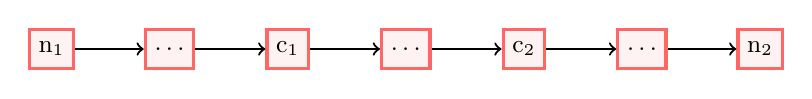
\begin{tikzpicture}[
node distance=1.5cm, thick, main/.style = {draw, circle},
squarednode/.style={rectangle, draw=red!60, fill=red!5, very thick, minimum size=5mm}]
\tikzstyle{every node}=[font=\small]
\node[squarednode] (1) {n$_{1}$}; 
\node[squarednode] (2) [right of=1] {$\hdots$};
\node[squarednode] (3) [right of=2] {c$_{1}$}; 
\node[squarednode] (4) [right of=3] {$\hdots$};
\node[squarednode] (5) [right of=4] {c$_{2}$};
\node[squarednode] (6) [right of=5] {$\hdots$};
\node[squarednode] (7) [right of=6] {n$_{2}$};

\draw[->] (1) -- (2);
\draw[->] (2) -- (3);
\draw[->] (3) -- (4);
\draw[->] (4) -- (5);
\draw[->] (5) -- (6);
\draw[->] (6) -- (7);
\end{tikzpicture} 
\end{center}
Using Observation 5.1.3, we can limit the number of nodes between any two facts in the final S$_{Q}$, therefore the final size of k will grow proportionally to q, but will still be exponential in w.

\subsection{5.2. Weaker notions of CQ-equivalence}
Let us define new versions of CQ-equivalence for sets of LTGD constraints $\Sigma_{1}$ and $\Sigma_{2}$, which constrain the sizes of the source instances D$_{0}$ or the sizes of the CQs Q:
\begin{enumerate}
	\item \textbf{j-CQ-equivalence}: $\forall$ instances D$_{0}$, CQ Q($\vec{x}$) consisting of j atoms, tuple $\vec{t}$ from D$_{0}$, D$_{0}$ $\wedge$ $\Sigma_{1}$ $\vDash$ Q($\vec{t}$) iff D$_{0}$ $\wedge$ $\Sigma_{2}$ $\vDash$ Q($\vec{t}$);
	\item \textbf{CQ-k-instance-equivalence}: $\forall$ instances D$_{0}$ containing k atoms, CQ Q($\vec{x}$), tuple $\vec{t}$ from D$_{0}$, D$_{0}$ $\wedge$ $\Sigma_{1}$ $\vDash$ Q($\vec{t}$) iff D$_{0}$ $\wedge$ $\Sigma_{2}$ $\vDash$ Q($\vec{t}$);
	\item \textbf{j-CQ-k-instance-equivalance}: $\forall$ instances D$_{0}$ of k atoms, CQ Q($\vec{x}$) consisting of j atoms, tuple $\vec{t}$ from D$_{0}$, D$_{0}$ $\wedge$ $\Sigma_{1}$ $\vDash$ Q($\vec{t}$) iff D$_{0}$ $\wedge$ $\Sigma_{2}$ $\vDash$ Q($\vec{t}$).
\end{enumerate}
Clearly, we get the following implications, for any j and k:
\begin{center}
\textbf{CQ-equivalence} $\Rightarrow$ \textbf{j-CQ-equivalence} $\Rightarrow$ \textbf{j-CQ-k-instance-equivalence}
\end{center}
\begin{center}
\textbf{CQ-equivalence} $\Rightarrow$ \textbf{CQ-k-instance-equivalence} $\Rightarrow$ \textbf{j-CQ-k-instance-equivalence}
\end{center}
\textbf{Proposition 5.2.1}: For sets of LTGDs $\Sigma_{1}$ and $\Sigma_{2}$, j-CQ-k-instance-equivalence is decidable.\newline
\textbf{Proof}: Enumerate all possible queries Q$_{j}$($\vec{x}$) of size j and instances D$_{k}$ of size k, fix a tuple $\vec{t}$ from the fixed source instance, and then we require to decide if the Boolean CQ Q$_{j}$($\vec{t}$) is entailed by D$_{k}$ and $\Sigma_{i}$, i $\in$ $\{$1,2$\}$, which by the Universality Theorem of the chase can be reduced to instances of Proposition 5.1.4. \newline
\textbf{Proposition 5.2.2}: The sets of LTGDs $\Sigma_{1}$ and $\Sigma_{2}$ are CQ-equivalent iff they are CQ-1-instance-equivalent.\newline
\textbf{Proof}: We will only prove the non-trivial implication. Suppose that $\Sigma_{1}$ and $\Sigma_{2}$ are CQ-1-instance-equivalent and let D be an arbitrary instance, Q($\vec{x}$) an arbitrary CQ, and $\vec{t}$ a tuple with constants from D. Suppose D $\wedge$ $\Sigma_{1}$ $\vDash$ Q($\vec{t}$), i.e. chase$_{\Sigma_{1}}$(D) $\vDash$ Q($\vec{t}$). Our goal is to show that chase$_{\Sigma_{2}}$(D) $\vDash$ Q($\vec{t}$). Let us write explicitly the form of the query:
\begin{center}
Q($\vec{t}$) = $\exists \vec{y}$ R$_{1}$($\vec{y_{1}}$,$\vec{t_{1}}$) $\wedge$ ... $\wedge$ R$_{n}$($\vec{y_{n}}$,$\vec{t_{n}}$)
\end{center}
where $\vec{y_{i}}$ $\subseteq$ $\vec{y}$ and $\vec{t_{i}}$ $\subseteq$ $\vec{t}$, 1 $\leq$ i $\leq$ n. Since chase$_{\Sigma_{1}}$(D) $\vDash$ Q($\vec{t}$), there must exist a valuation $\vec{a}$ for the existential variables in Q such that chase$_{\Sigma_{1}}$(D) contains all facts R$_{i}$($\vec{a_{i}}$,$\vec{t_{i}}$). Each such fact was generated from exactly one fact from D (and its creation solely depends on that fact, independently on the other branches created from D), as the bodies of all LTGDs have a single atom. For each such fact R$_{i}$($\vec{a_{i}}$,$\vec{t_{i}}$), let D$_{i}$ be the substructure of D containing just the fact that generated it. Also, for each atom in Q($\vec{t}$), let 
\begin{center}
Q$_{i}$($\vec{t_{i}}$) = $\exists \vec{y_{i}}$ R$_{i}$($\vec{a_{i}}$,$\vec{t_{i}}$)
\end{center}
Then, chase$_{\Sigma_{1}}$(D$_{i}$) $\vDash$ Q$_{i}$($\vec{t_{i}}$) and by CQ-1-instance-equivalence, chase$_{\Sigma_{2}}$(D$_{i}$) $\vDash$ Q$_{i}$($\vec{t_{i}}$). Thus, since chase$_{\Sigma_{1}}$(D) is formed from all the chases executed on the single-fact instances, we can combine all the homomorphisms for the smaller queries to create a homomorphism for Q($\vec{t}$), which proves that chase$_{\Sigma_{2}}$(D) $\vDash$ Q($\vec{t}$).\newline
This result limits the space we need to search for CQ-equivalence, as now we only need to check for single-atom instances D$_{0}$.

\newpage

\section{6. Conclusions}
\subsection{6.1. Summary}
The project has largely achieved the desired goals outlined in the project description. We have gradually introduced the reader to the background necessary for stating our contributions, which are:
\begin{itemize}
	\item two new types of equivalences for schema mappings, together with their relation with respect to the already existing ones;
	\item study and prove decidability of chase compatibility for special classes of constraints;
	\item use automata approach to obtain lower complexity bounds for the decidability checking mentioned previously;
	\item study relaxed versions of CQ-equivalence and prove decidability results on them.
\end{itemize}
\subsection{6.2. Related work}
The closest reference to what is discussed in this project is \cite{equivalence}, which analyses the decidability of the equivalence types defined in Section 3.1 (without the new ones). Another closely related work comes from \cite{theory}.
\subsection{6.3. Future directions}
One extension for the decidability results for would be to relax the constraints imposed on the class of dependencies that we work with. It would be challenging to also generalize the use of automata in Section 4.4 for multi-headed LTGDs. Another question would be about the necessity of all the rules imposed in Theorem 3.2.1.

\newpage

\begin{thebibliography}{9}

\bibitem{decidable}
Michael Benedikt, Michael Vanden Boom. \emph{\href{http://www.cs.ox.ac.uk/michael.benedikt/readingcourse/coursenotes2020.pdf}{Decidable Logics via Automata}} (pg. 30-46).

\bibitem{modern}
Michael Benedikt, Balder ten Cate. \emph{\href{https://cpb-us-e1.wpmucdn.com/sites.ucsc.edu/dist/4/1230/files/2014/09/esslli-all.compressed.pdf} {Modern Database
Dependency Theory}} (slides 79-84).

\bibitem{klug}
D.S. Johnson, A. Klug. \emph{\href{https://cs.uwaterloo.ca/~david/kbdb/johnstonandklug.pdf}{Testing containment of conjunctive queries under functional and inclusion dependencies}}.

\bibitem{dataexchange}
Ronald Fagin, Phokion G. Kolaitis, Renée J. Millerc,
Lucian Popa. \emph{\href{http://dblab.cs.toronto.edu/project/dataexchange/docs/tcs05.pdf}{Data exchange: semantics and query answering}}.

\bibitem{dataintegration}
Maurizio Lenzerini. \emph{\href{https://tanca.faculty.polimi.it/wp-content/uploads/images/documents/TIS/lezioni/1_3_integration-lenzerini.pdf}{Data Integration: A Theoretical Perspective}}.

\bibitem{equivalence}
Reinhard Pichler, Emanuel Sallinger, Vadim Savenkov. \emph{\href{http://www.dit.unitn.it/~p2p/RelatedWork/Matching/a10-pichler.pdf}{Relaxed Notions of Schema Mapping Equivalence Revisited}}.

\bibitem{theory}
Ronald Fagin, Phokion Kolaitis, Alan Nash
, Lucian Popa. \emph{\href{https://www.researchgate.net/publication/221559365_Towards_a_theory_of_schema-mapping_optimization}{Towards a theory of schema-mapping optimization}}.

\bibitem{trigger}
Efthymia Tsamoura, David Carral, Enrico Malizia, Jacopo Urbani.\emph{\href{http://www.vldb.org/pvldb/vol14/p943-tsamoura.pdf}{Materializing Knowledge Bases via Trigger Graphs}}.

\end{thebibliography}

\end{document}
